\appendix

\section{Appendix A: Examples of DWARF entries}
\begin{figure}[ht]
    \centering
    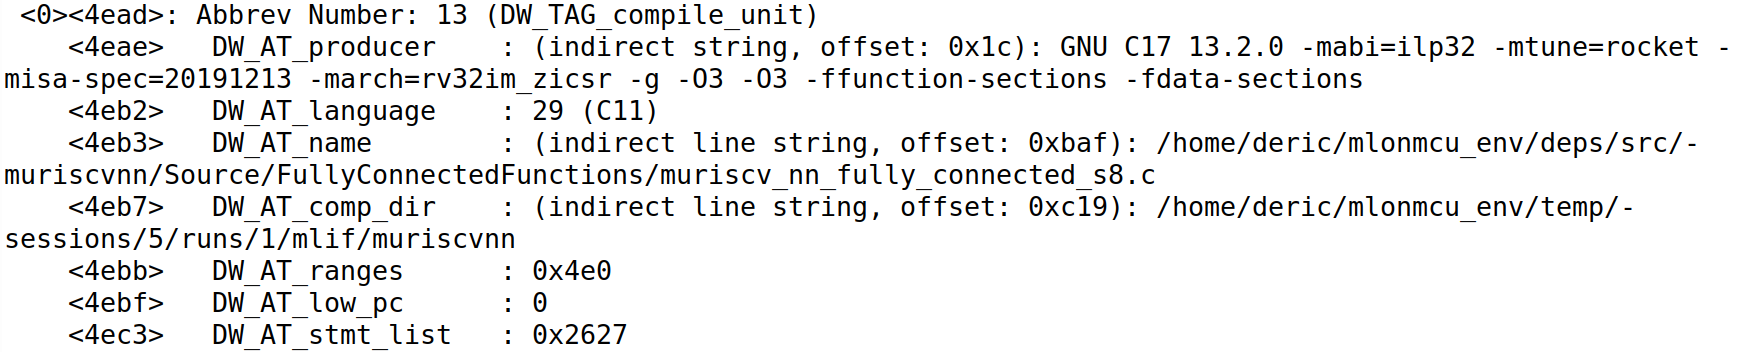
\includegraphics[width=.95\linewidth]{figures/DWARF_compile_unit.png}
    \caption{Example of DWARF compile unit}
    \label{fig:dwarf_compile_unit}
\end{figure}

\begin{figure}[ht]
    \centering
    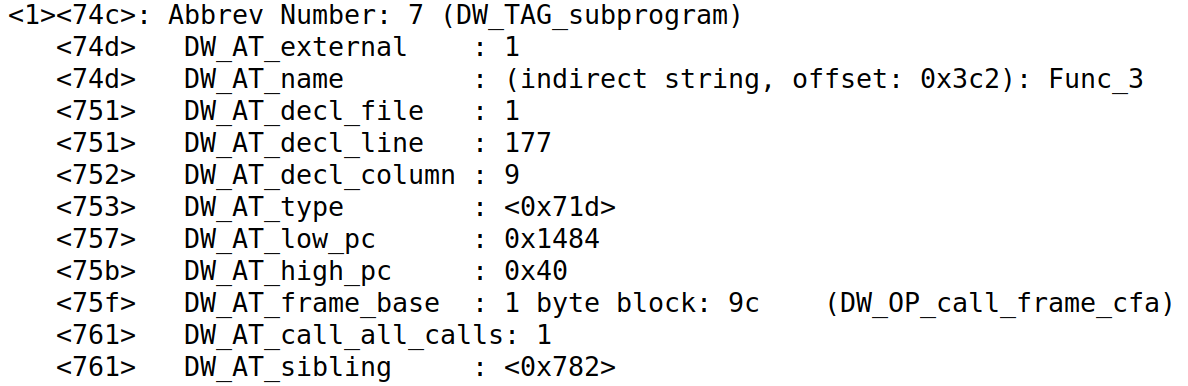
\includegraphics[width=.95\linewidth]{figures/DWARF_subprogram.png}
    \caption{Example of DWARF subprogram}
    \label{fig:dwarf_subprogram}
\end{figure}

\begin{figure}[ht]
    \centering
    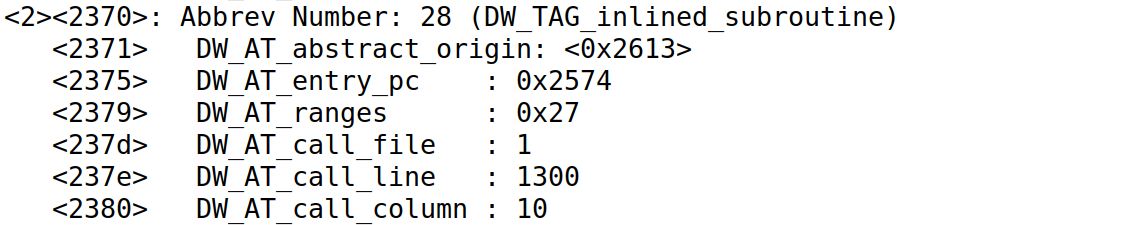
\includegraphics[width=.95\linewidth]{figures/DWARF_inlined_subroutine.png}
    \caption{Example of DWARF inlined subroutine}
    \label{fig:dwarf_inlined_subroutine}
\end{figure}

\begin{figure}[ht]
    \centering
    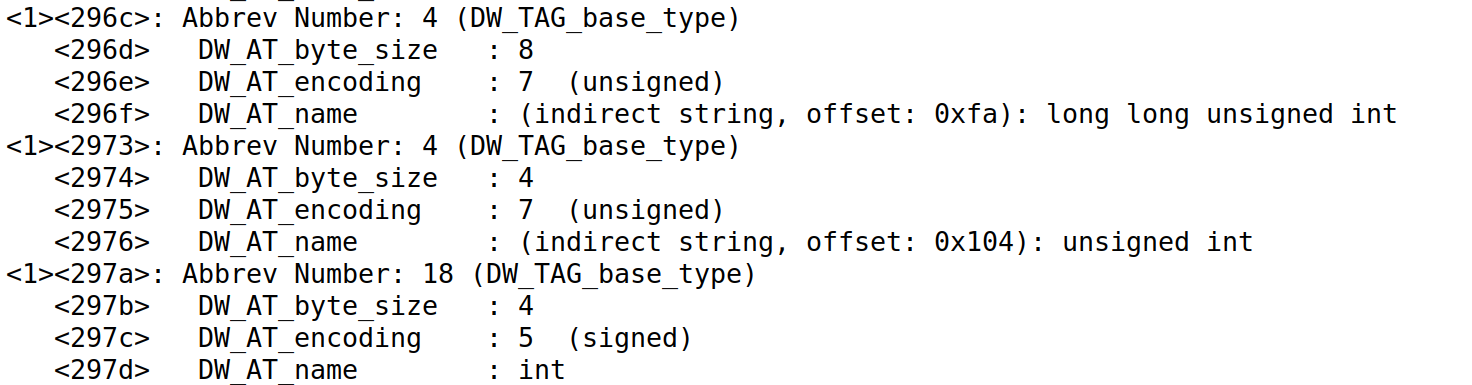
\includegraphics[width=.95\linewidth]{figures/DWARF_base_type.png}
    \caption{Example of DWARF base type}
    \label{fig:dwarf_base_type}
\end{figure}

\begin{figure}[ht]
    \centering
    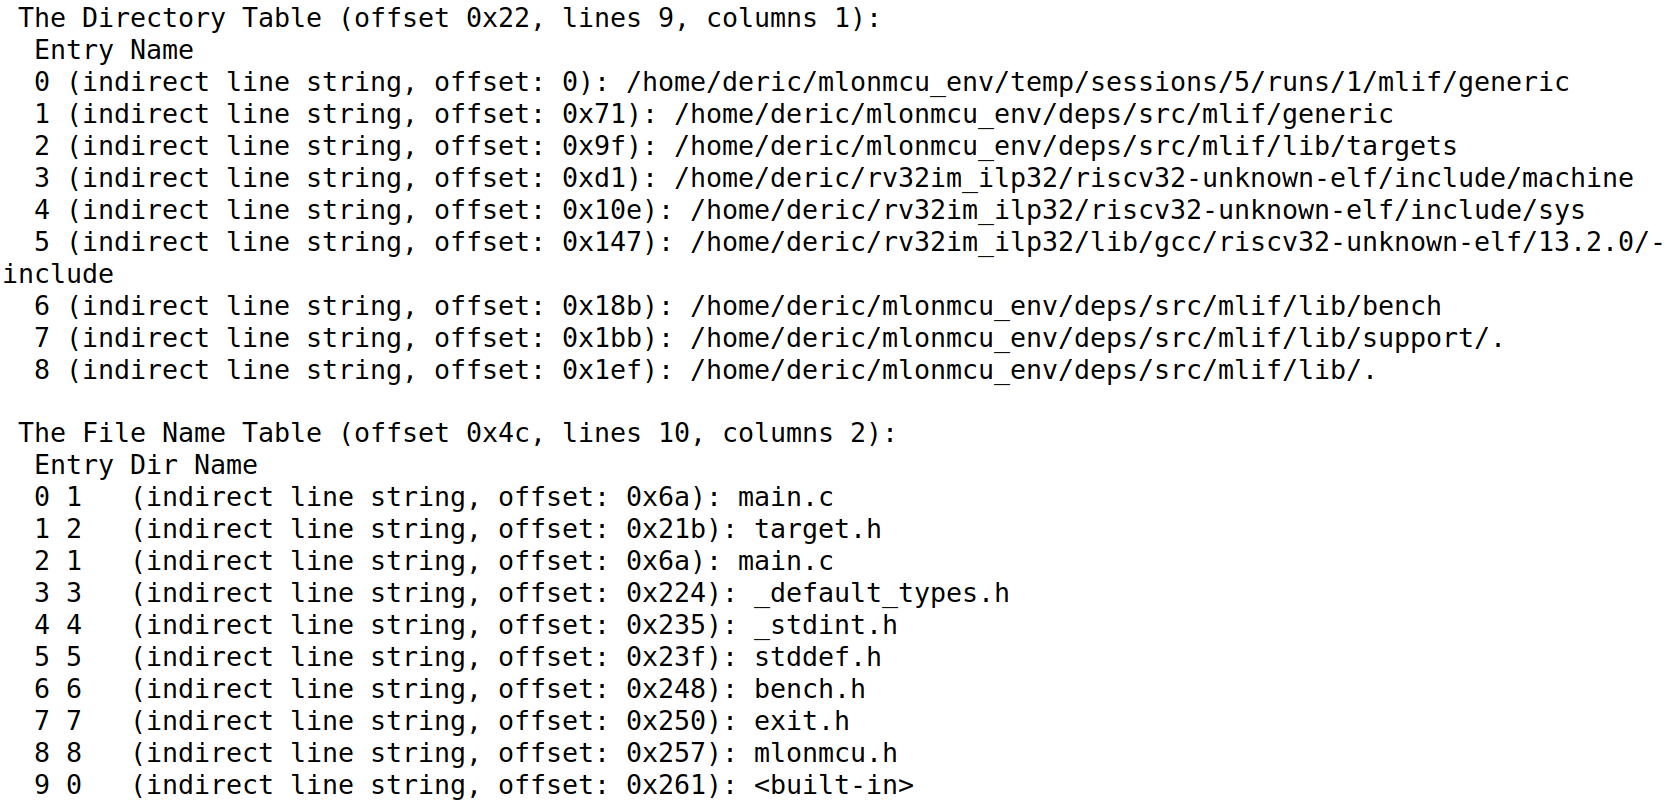
\includegraphics[width=.95\linewidth]{figures/DWARF_debug_prologue.png}
    \caption{Example of DWARF directory table and file name table}
    \label{fig:dwarf_debug_prologue}
\end{figure}

\begin{figure}[ht]
    \centering
    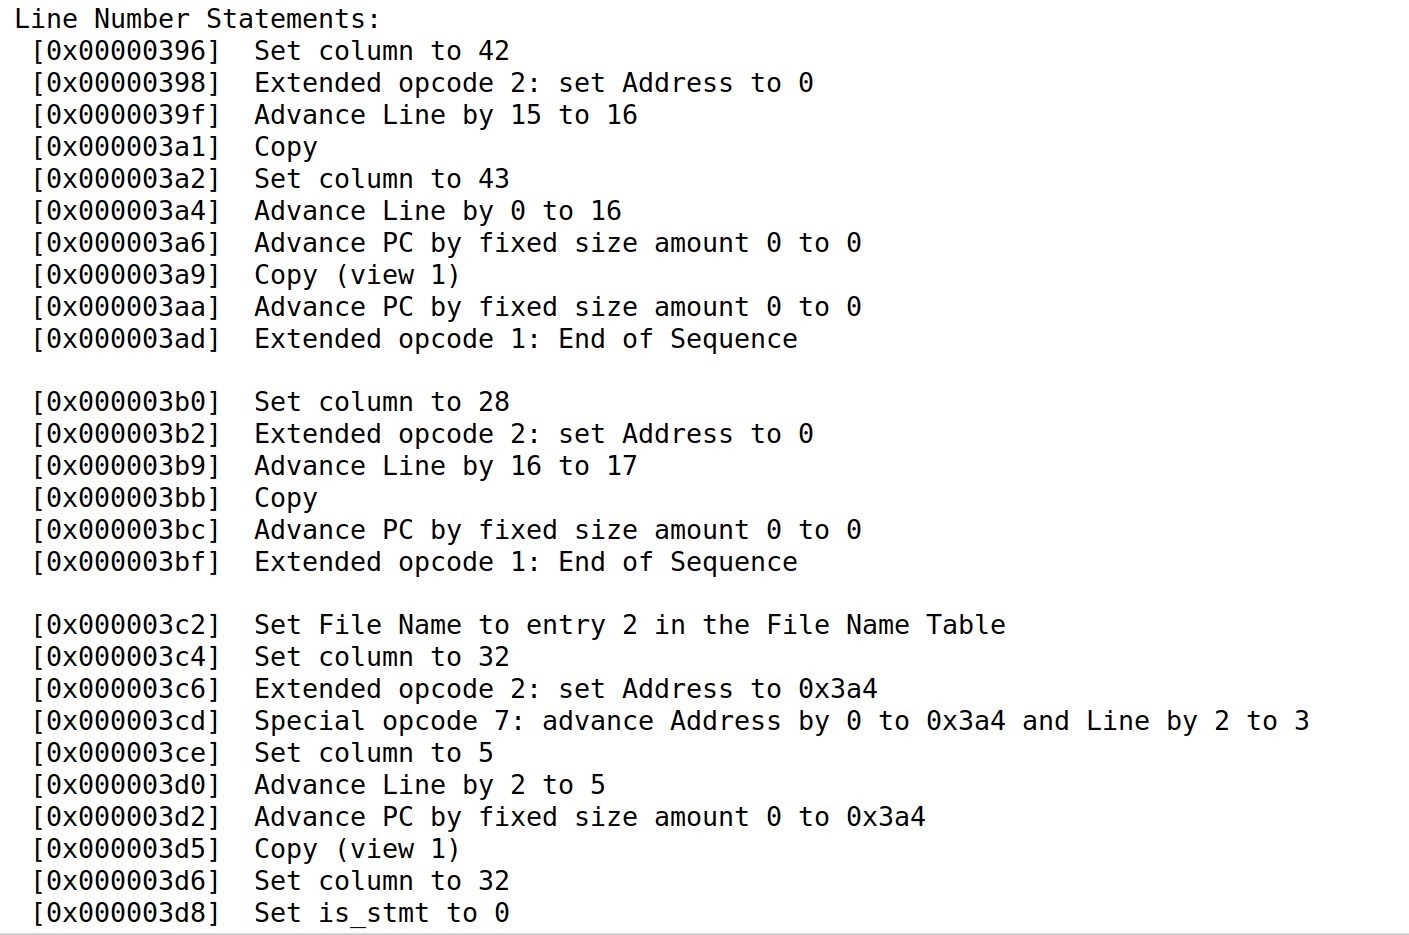
\includegraphics[width=.85\linewidth]{figures/DWARF_debug_main.png}
    \caption{Example of DWARF line number statement}
    \label{fig:dwarf_debug_main}
\end{figure}

\section{Appendix B: Implementation code snippets}
\begin{center}
\begin{minipage}{\textwidth}
\lstset{caption={Helper function for retrieving the file name}, label=code:helper_function}
\begin{lstlisting}
def lpe_filename(line_program, file_idx):
    lp_header = line_program.header
    file_entries = lp_header['file_entry']

    file_entry = file_entries[file_idx] if line_program.header.version >= 5 else \
        file_entries[file_idx-1]
    dir_idx = file_entry['dir_index'] if line_program.header.version >= 5 else \
        file_entry['dir_index'] - 1

    if dir_idx == 0:
        return file_entry.name.decode()

    directory = lp_header['include_directory'][dir_idx]
    return posixpath.join(directory, file_entry.name).decode()
\end{lstlisting}
\end{minipage}
\end{center}


\medskip
\begin{center}
\begin{minipage}{\textwidth}
\lstset{caption={Naive Implementation of \texttt{func\_name} query function}, label=code:naive_implementation}
\begin{lstlisting}
# Assume pc_to_func_mapping is given
# pc_to_func_mapping: {func_name : (start_pc, end_pc)}

def find_func_name(pc: int) -> str:
    for func_name, range in pc_to_func_mapping.items():
        if range[0] <= pc <= range[1]:
            return func_name
    return "???"

\end{lstlisting}
\end{minipage}
\end{center}

\begin{center}
\begin{minipage}{\textwidth}
\lstset{caption={Implementation of \texttt{func\_name} query function by using binary search}, label=code:binary_search_func_name}
\begin{lstlisting}
import bisect

# pc_to_func_mapping is now a list and
# is sorted in ascending order based on start_pc
# pc_to_func_mapping: (start_pc, end_pc, func_name) 
# pc_to_func_mapping.sort(key=lambda x : x[0])

def find_func_name(pc: int) -> str:
    i = bisect.bisect_right(pc_to_func_mapping, pc, key=lambda x : x[0])
    if i > 0:
        start_pc, end_pc, func_name = pc_to_fun_mapping[i-1]
        if start_pc <= pc <= end_pc:
            return func_name
    return "???"
    
\end{lstlisting}
\end{minipage}
\end{center} 

\begin{center}
\begin{minipage}{\textwidth}
\lstset{caption={Implementation of source line query function by using binary search}, label=code:binary_search_source_line}
\begin{lstlisting}
import bisect

# pc_to_source_line_mapping : {source_file : [(pc, source_line), ...]}
# Asssume pc_to_source_line_mapping is given and
# , for each source file, the list is sorted in ascending order
# based on pc

def dump_source_line(pc: int, source_file: str) -> str:
    if source_file == "???":
        return "0"
    mapping = pc_to_source_line_mapping[source_file]
    i = bisect.bisect_right(mapping, pc, key=lambda x : x[0])
    if i > 0:
        start_pc, line = mapping[i-1]
        if pc >= start_pc:
            return f"{line}"
    return "0"

\end{lstlisting}
\end{minipage}
\end{center}

\section{Appendix C: Callgraph of benchmarks}
\begin{figure}[ht]
    \centering
    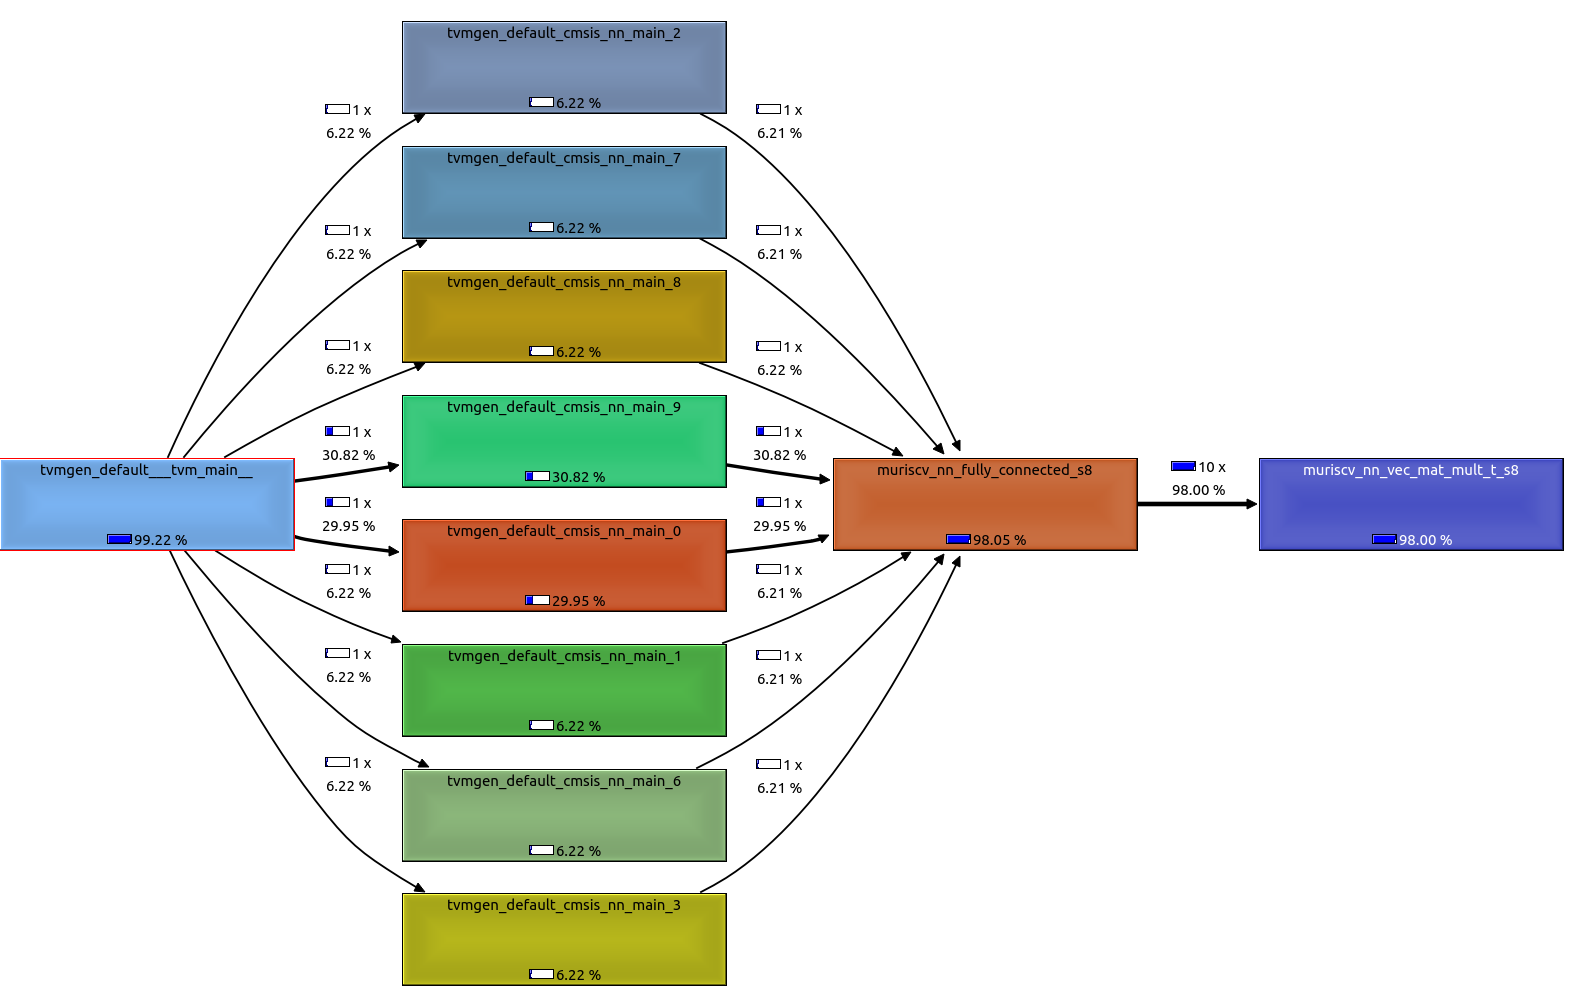
\includegraphics[width=.9\linewidth]{figures/evaluation_toycar_call_graph.png}
    \caption{Callgraph of toycar benchmark in kcachegrind}
    \label{fig:evaluation_toycar_call_graph}
\end{figure}

\begin{figure}[ht]
    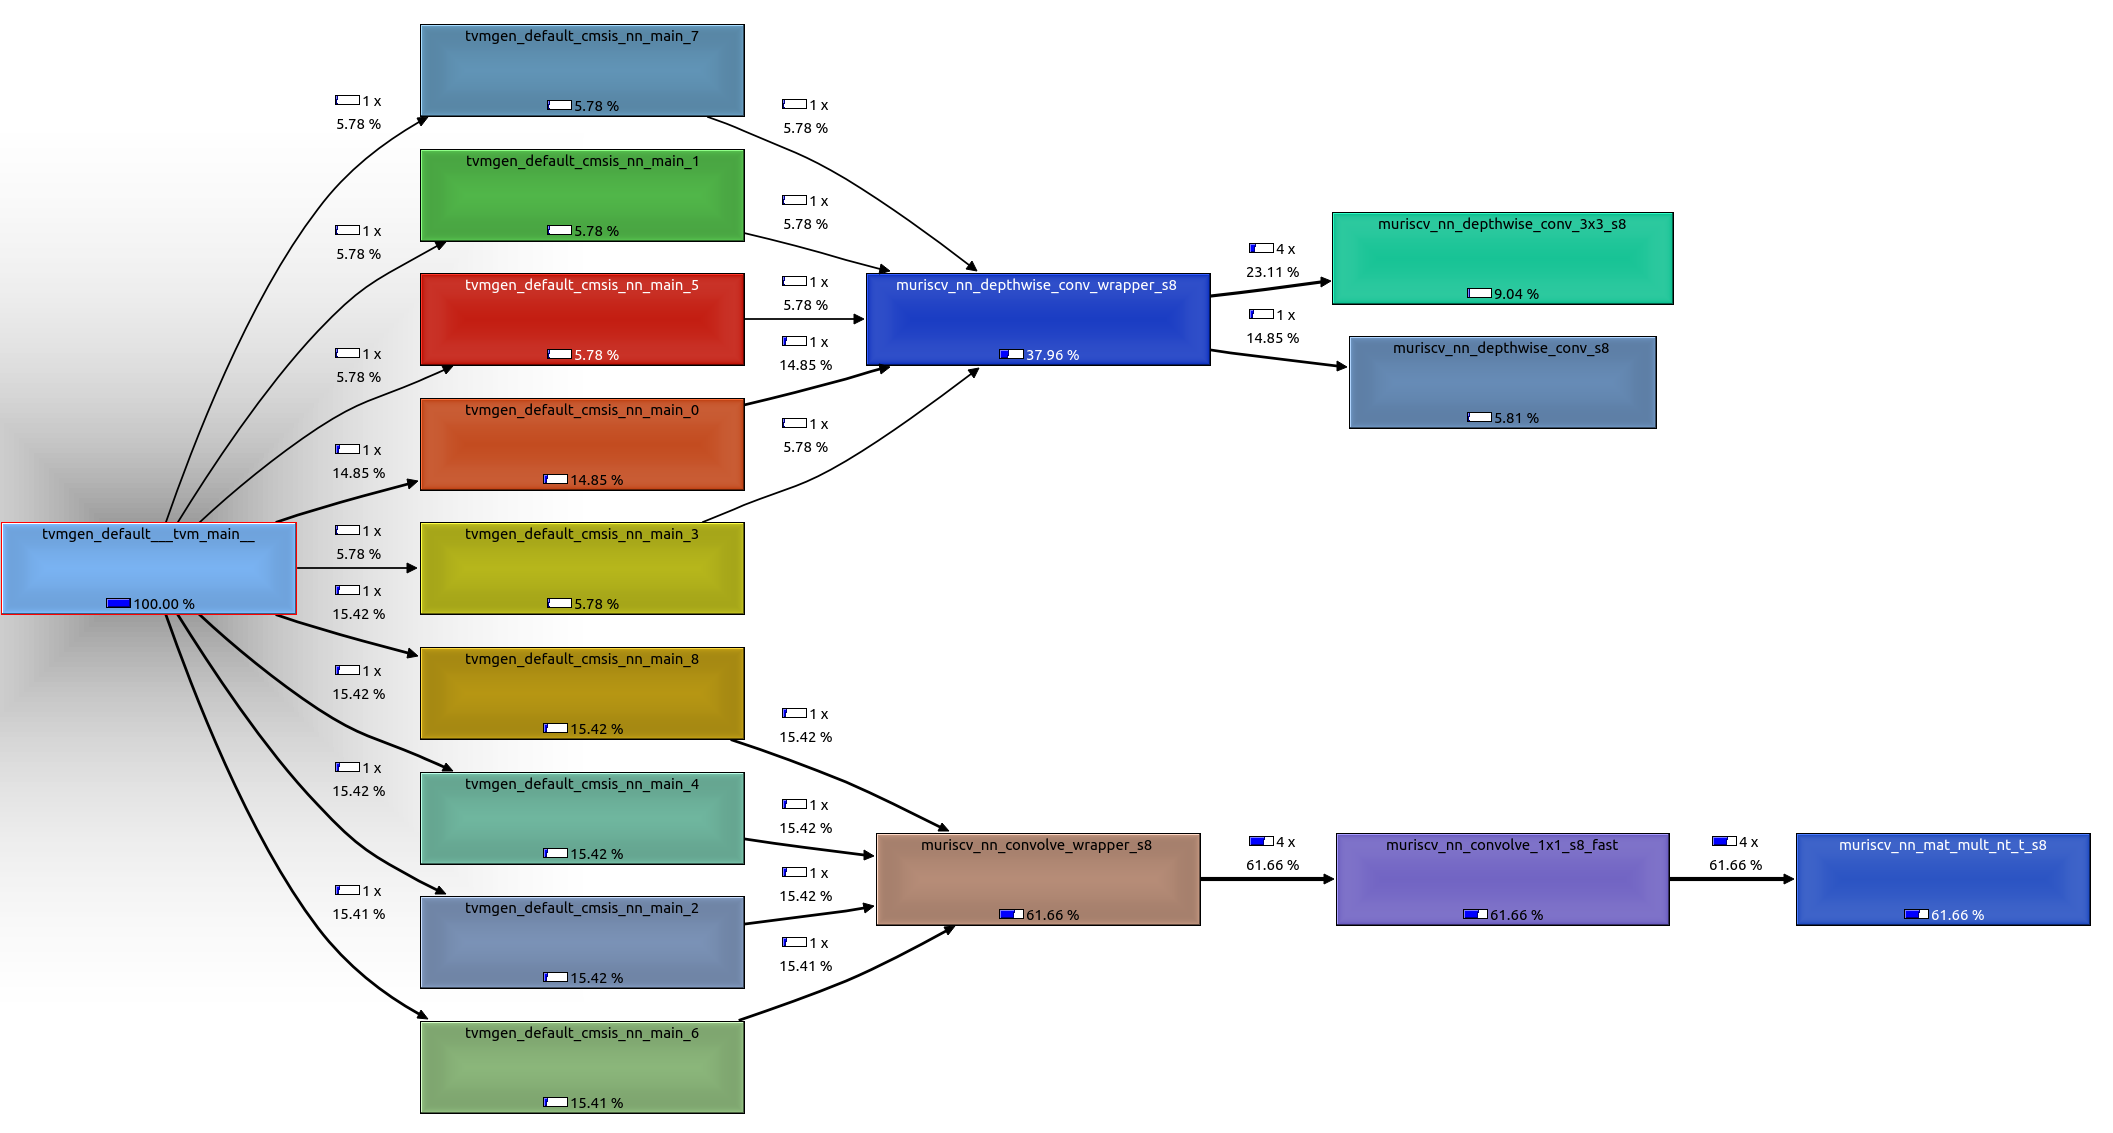
\includegraphics[width=\linewidth]{figures/evaluation_aww_call_graph.png}
    \caption{Callgraph of aww benchmark in kcachegrind}
    \label{fig:evaluation_aww_call_graph}
\end{figure}

\begin{figure}[ht]
    \centering
    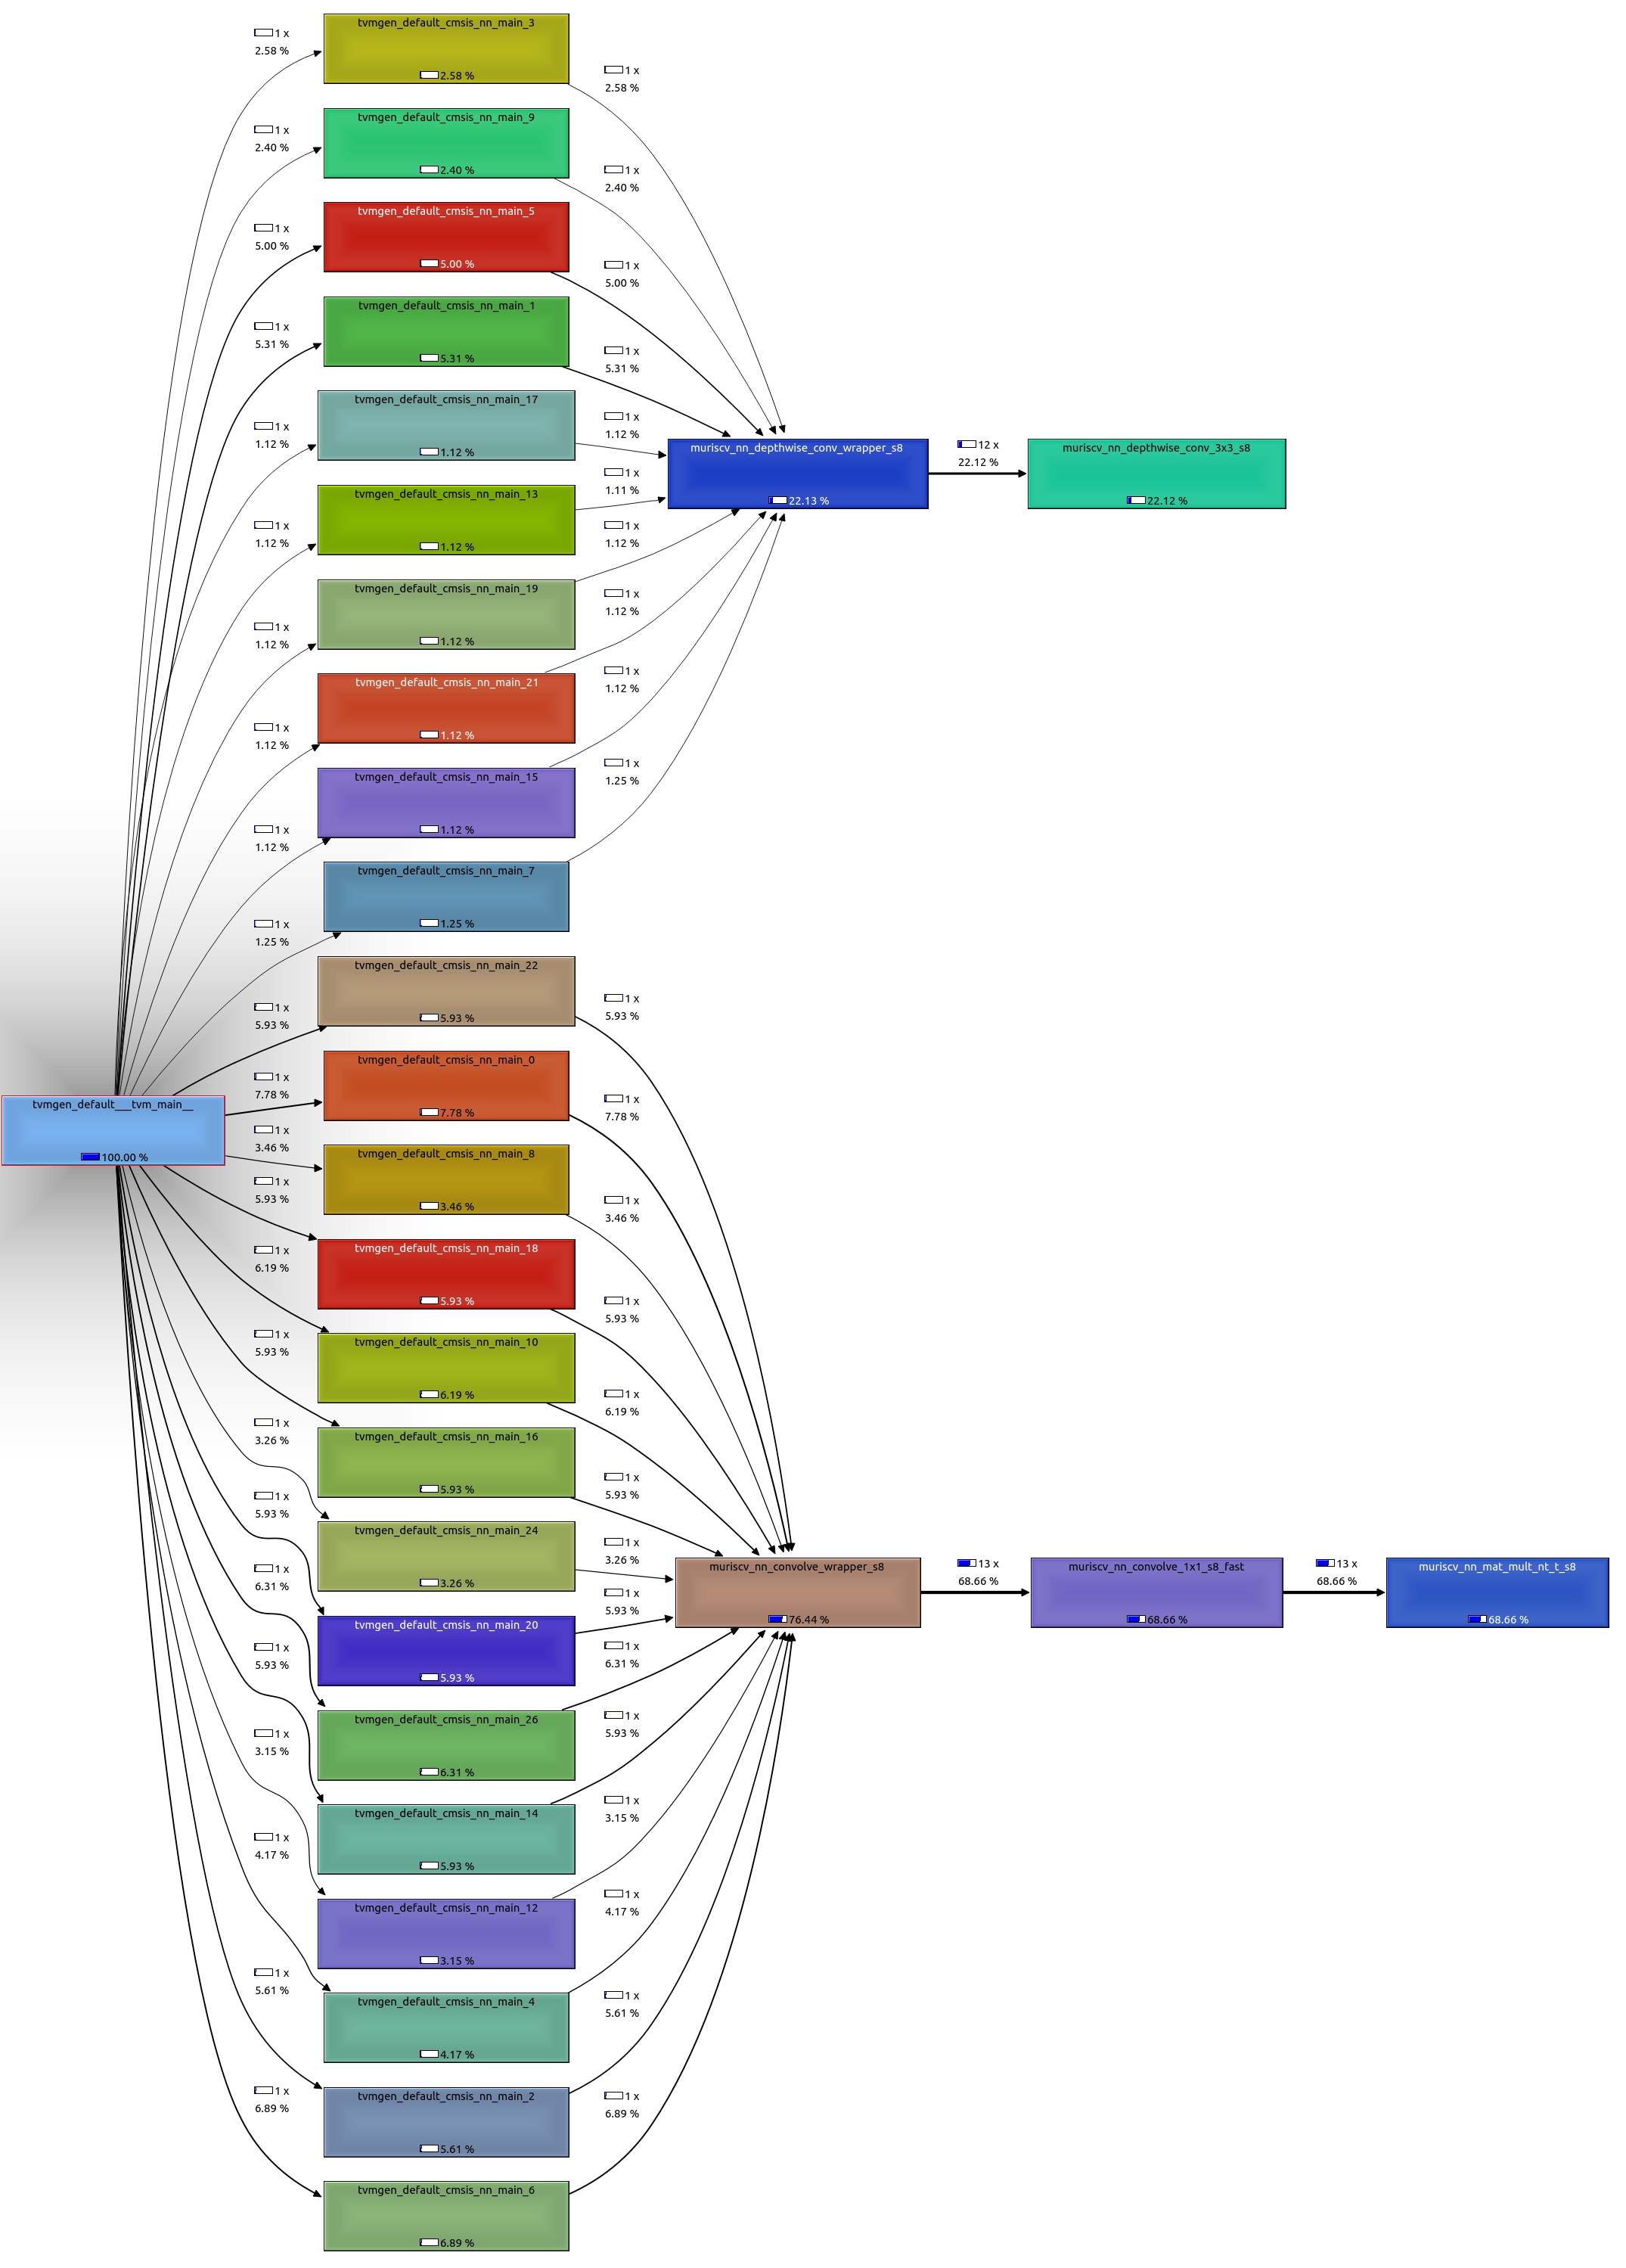
\includegraphics[width=.9\linewidth]{figures/evaluation_vww_call_graph.png}
    \caption{Callgraph of vww benchmark in kcachegrind}
    \label{fig:evaluation_vww_call_graph}
\end{figure}

\begin{figure}[ht]
    \centering
    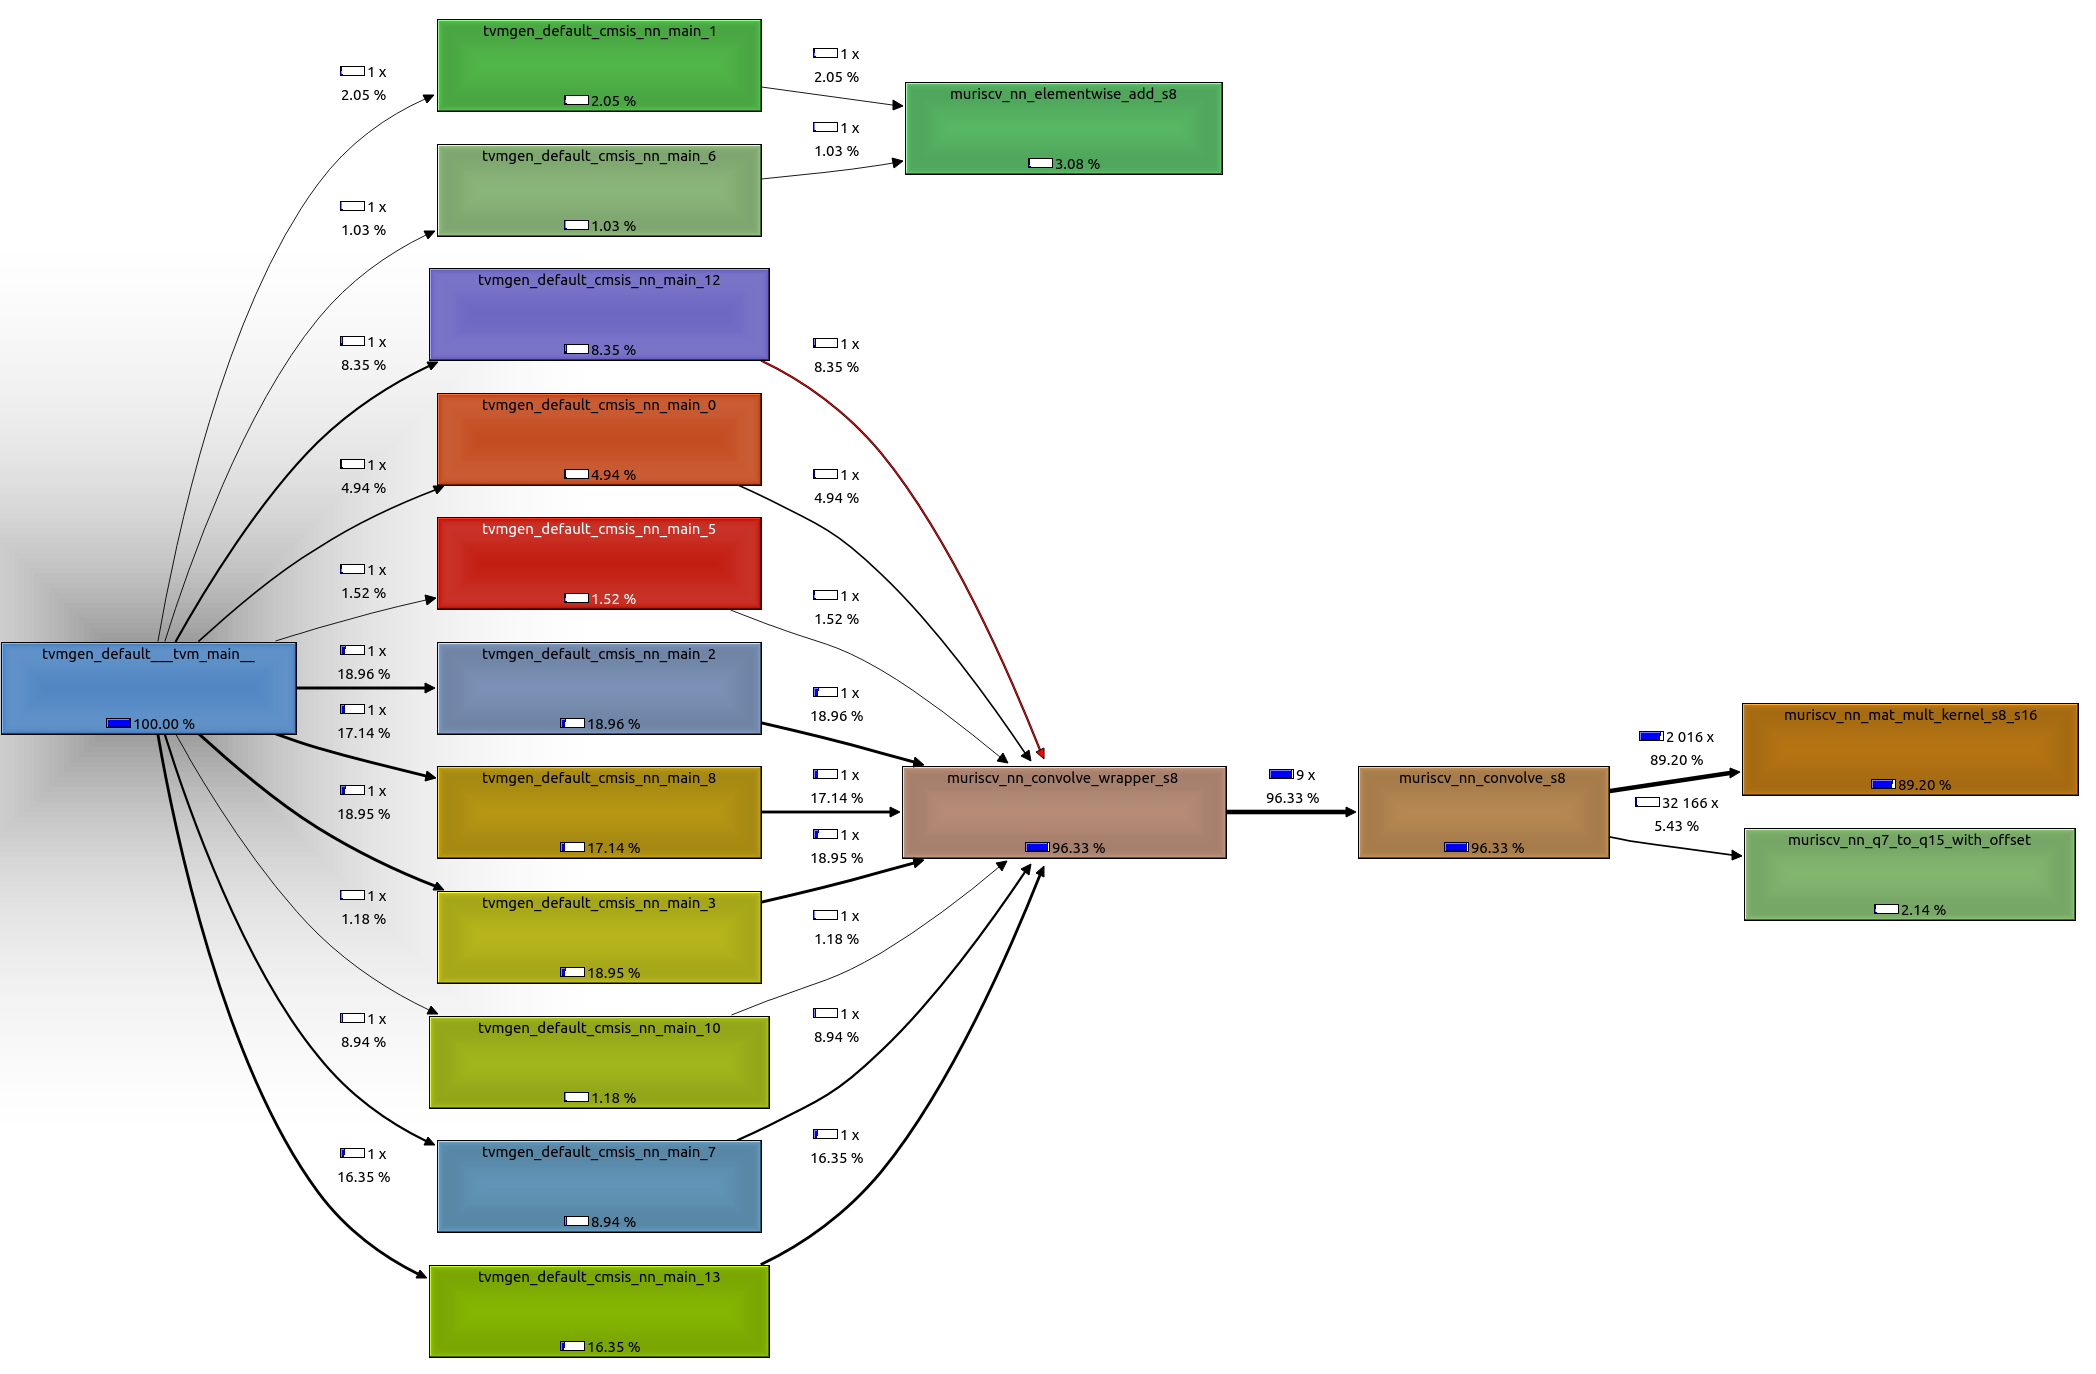
\includegraphics[width=.9\linewidth]{figures/evaluation_resnet_call_graph.png}
    \caption{Callgraph of resnet benchmark in kcachegrind}
    \label{fig:evaluation_resnet_call_graph}
\end{figure}